\pc{2}{7/2}

\question A building is modelled as a grid.
People stand on $m$ points of the grid,
and all these people have to be able to leave the building in case of emergency (e.g. fire).
Therefore they have to be able to reach a vertex on the border of the grid through some path.
It is not allowed that two emergency exit-paths share any vertex.
The following picture illustrates an example of such an emergency exit plan:
\begin{center}
    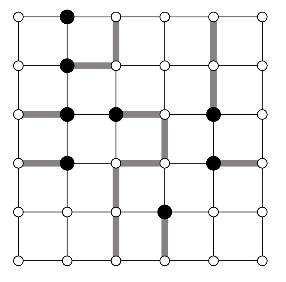
\includegraphics[width=0.4\textwidth]{images/pc-02-1.png}
\end{center}
Model this emergency exit problem as a maximum flow problem.

\question Let $N=(G,c,s,t)$ be a flow network and assume that $N$ admits a non-zero flow.
Show that there exists at least one edge $e$ in $N$ whose removal decreases the vallue of a
maximum flow in $N$.
An edge $e$ is called \emph{most vital} if the removal of $e$ decreases the maximum flow as much as possible.
Is an edge of maximum capacity in a minimal cut necessarily most vital?

\question 
Within a sensor network, sensors receive data that are later collected at a central node of the network.
We now want to chech whether these data can be collected at the central node within $T$ steps.
Formally we consider the following problem.

Let $G = (V,E)$ be a directed graph with $n$ vertices and $m$ edges and let $t \in V$ be a sink 
(corresponding to the \emph{central node} of the network).
Every vertex $v \in V \setminus \{t\}$ has a data packet $p_v$ which has to be transmitted to the sink $t$.
To do that, the packet $p_i$ may have to be forwarded through several other vertices of the graph.
We assume that there exists a central clock on the network, which synchronises all activities of the vertices.
At time point $t$ every vertex can send a data packet through an out-going edge.
This transmission of the data packet over one edge takes exactly 1 unit of time to be performed (e.g. 1ms).
Simulateneously, at any time, every vertex can receive data packets from an abitrary number of incoming edges.

Model the following decision problem as a maximum flow problem: 
\emph{can we send the data packets through the network such that all packets arrive at sink $t$ with $T$ time units?}
(Hint: construct a flow network with $2T(n-1) + 2$ vertices.)

\question Consider the following variants of \textsc{Vertex-Cover}:
\begin{enumerate}
    \item DVC - decision variant: 
        \emph{does there exist a vertex cvover of cardinality $k$?};
    \item OVC - optimisation variant:
        \emph{which is the cardinality of a minimum vertex cover?}; and
    \item \textsc{Min}VC - construct of the solution:
        \emph{find a smallest vertex cover and output it.}
\end{enumerate}
Prove that all these variants can be reduced to each other in polynomial time.
\begin{parts}
    \part Assume that you have an algorithm for DVC with running time $\operatorname{poly}(n)$.
    Give a polynomial-time algorithm for OVC>

    \part Assume that you have an algorithm for OVC with running time $\operatorname{poly}(n)$.
    Give a polynomial-time algorithm for $\textsc{Min}VC$.
\end{parts}
Show that correctness and justify why the constructed algorithms have polynomials running time.
